% Source: graduate-coursework/Research/Papers/drafts/temporal_context_motion_trails/Radar_TemporalContext_MotionTrails.tex
% Description: Accuracy--horizon curves showing an optimal medium trail length and degradation under long trails.

\documentclass[border=4pt]{standalone}
\usepackage{algpseudocode}
\usepackage{amsmath,amssymb}
\usepackage[T1]{fontenc}
\usepackage{pgfplots}
\usepackage{tikz}
\usepackage{xcolor}
\pgfplotsset{compat=1.18}
\usetikzlibrary{arrows.meta,positioning,calc,fit,shapes.geometric,shapes.misc,decorations.pathmorphing,backgrounds}


\newcommand{\ph}[1]{\textcolor{red}{#1}}

\begin{document}
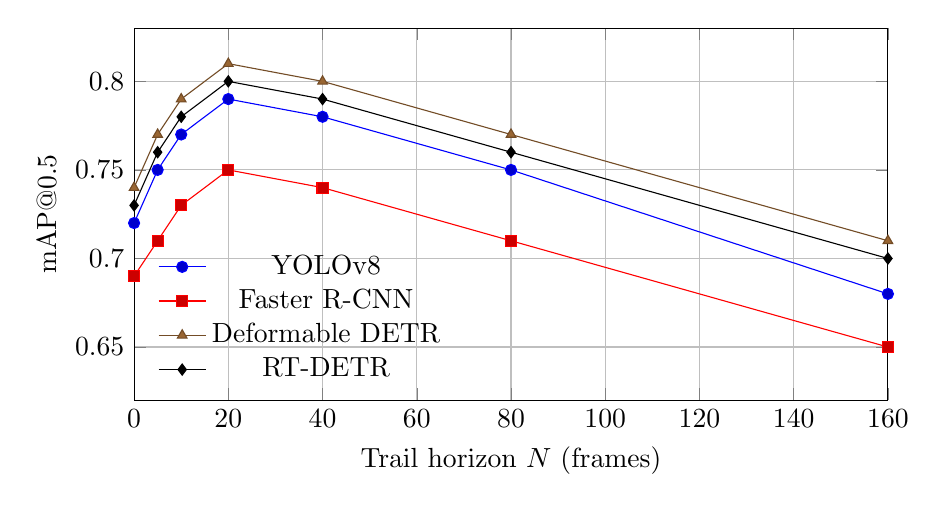
\begin{tikzpicture}
\begin{axis}[
  width=0.92\linewidth,
  height=0.52\linewidth,
  xlabel={Trail horizon $N$ (frames)},
  ylabel={mAP@0.5},
  xmin=0, xmax=160,
  ymin=0.62, ymax=0.83,
  grid=both,
  legend style={at={(0.02,0.02)},anchor=south west,draw=none,fill=none},
]
\addplot+[mark=*] coordinates {(0,0.72) (5,0.75) (10,0.77) (20,0.79) (40,0.78) (80,0.75) (160,0.68)};
\addlegendentry{YOLOv8}
\addplot+[mark=square*] coordinates {(0,0.69) (5,0.71) (10,0.73) (20,0.75) (40,0.74) (80,0.71) (160,0.65)};
\addlegendentry{Faster R-CNN}
\addplot+[mark=triangle*] coordinates {(0,0.74) (5,0.77) (10,0.79) (20,0.81) (40,0.80) (80,0.77) (160,0.71)};
\addlegendentry{Deformable DETR}
\addplot+[mark=diamond*] coordinates {(0,0.73) (5,0.76) (10,0.78) (20,0.80) (40,0.79) (80,0.76) (160,0.70)};
\addlegendentry{RT-DETR}
\end{axis}
\end{tikzpicture}
\end{document}
